%% Marco Teórico C2 %%

\chapter{Teoría Funcional}

Llamamos programación funcional a un paradigma de computación, el cual comenzó a principios de los sesenta, impulsado por las necesidades de científicos de la inteligencia artificial de comprender y programar los procesos del cálculo simbólico, teoría de pruebas y pruebas de teoremas ya en tal época ningún lenguaje imperativo daba una aproximación a estas necesidades.\\
La programación funcional trata los cálculos como funciones matemáticas, no existe la noción de posición de memoria, por tanto tampoco de asignación, a través de la aplicación de los teoremas de recursividad se operan los bucles, también se distingue la notación frente a lenguajes imperativos clásicos. Hoy en día, algunos lenguajes de programación han tratados de implementar este paradigma.\\
La programación funcional se cimenta en el cálculo lambda desarrollado por Church en los treinta para dar una teoría paralela de funciones, este provee a la programación de sintaxis, semántica para definir función y permite definir primitivas de programación.

\section{Lenguajes funcionales}

\subsection{Funciones}

Antes de que los ordenadores vieran la luz se habian concedido tecnicas para solucionar problemas. Por tanto la terminologia referente a memoria no se usaba. En la matemática un concepto fundamental  es el de función, las cuales actuan como un procesador con una entrada y dando como resultado una salida, los resultados dependen de los parametros a traves de cada pasó, es por eso que se puede asociar una función, con la computación.\\

Podemos entonces decir que un ``programa'' consiste en la definicion de una o varias funciones.  el ordenador procesa los parametros en la funcion  entrega el resultado. Con esta aproximacion no tenemos que preocuparnos del orden de ejecucion, lo cual ya es mas potente que la aproximacion imperativa.
Al pasar el tiempo evidentemente esta tendencia fue perdiendo fuerza en el mercado pero nunca en la academia 

\subsection{Lenguajes}

A finales de los cincuenta John McCarthy creo el primer lenguaje de programación funcional Lisp. Posteriormente y por la necesidad de dar mas fortaleza al tipado se crearon otros, ML, Scheme, Hope. Cada investigador se enfocaba en crear el suyo propio, tratando de tomar lo mejor de cada uno, un grupo de cientificos de la computacion creo Haskell en los noventa. Posteriormente vendrian versiones de los que ya existian y algunos nuevos Clojure, Scala entre otros, algunos ya tomando fuerza en desarrollos empresariales, por ejemplo F\#.

\subsection{Teoria de Categorias y Programación Funcional}

Muchos conceptos de ka programación funcional tienen su origen en la teoria de categorias, por ello introducimos a partir de ahora esta teoria de manera formal como sustento axiomatico de nuestro trabajo.

\subsection{Definiciones formales en Teoria de Categorias}

\begin{note}\end{note}
\begin{itemize}
\item Usamos $:$ para definir tipos, asumimos implicitamente el tipado para evitar sobrecargar la notacion cuando no haya confusión al respecto, de lo contrario se escribe $.$ antecedido del tipo.
\item $\Omega$ es uns generalización para los tipos, es decir el contenedor universal de tipos
\item $\Sigma_{\Omega}$ es el conjunto contenedor, se infiere de su contexto
\item El signo $:$ representa el alcance de los cuantificadores si se ubica despues de uno de estos, de lo contrario representa una definicion
\end{itemize}

\begin{defn}[Monoide]
\end{defn}
Tupla $\langle M, *, \mft{a}, e, \mft{i} \rangle$ 
\begin{itemize}
\item Conjunto $M: \Omega$
\item Operador $* : M \times M \to M$
\item Asociatividad $\mathcal{a} : \forall_{m_1, m_2, m_3 \in M} ((m_1 * m_2) * m_3 = m_1 * (m_2 * m_3))$
\item $e$ Elemento Identidad [$\mft{i}$] $\forall_{m \in M} ( e * m = m = m * e)$
\end{itemize}

\begin{defn}[Agregación]
\end{defn}
Tupla $\langle M, \Pi, \mft{a}, \mft{i} \rangle$  
\begin{itemize}
\item Conjunto $M: \Omega$ 
\item Agregador $\Pi: \mathcal{L} M \to M$
\item Asociatividad $\mft{a}: \forall_{ n \in \mathbb{N}, \vec{m_1}, \dots, \vec{m_n} \in \mathcal{L}M}
(\prod [\prod \vec{m_1}, \dots , \prod \vec{m_n}] = \prod(\vec{m_1} ++ \dots ++ \vec{m_n}))$
\item Identidad $i: \forall_m ( m = \Pi[m])$
\end{itemize}

\begin{defn}[Homomosfismos de Monoides de $\langle M, *, e \rangle$ hacia $\langle N, +, i \rangle$]
\end{defn}
Tupla $\langle f, \mft{d}, \mft{i} \rangle$ 
\begin{itemize}
\item Función $f : M \to N$ 
\item Distributividad $\mft{d} : \forall_{m_1, m_2}( f(m_1) + f(m_2) = f(m_1 * m_2))$
\item Identidad ${i} : i = f(e)$
\end{itemize}

\begin{defn}[Homomosfismo de Monoides]
\end{defn}
Es una tupla $\langle f, \mft{d} \rangle$ basada en una aplicación de $\langle M, \Pi \rangle$ hacia $\langle N, \Sigma \rangle$  
\begin{itemize}
\item Función $f: M \to N$
\item Distributividad $\mft{d} : \forall_{ n \in \mathbb{N}, m_1, \dots, m_n }( \Sigma \left[f(m_1), \dots, f(m_n)\right] = f\left(\Pi \left[m_1, \dots, m_n\right]\right))$
\end{itemize}

\begin{note}
En general denotamos homomorfismo como  $\hom$
\end{note}

\begin{defn}[Categoria]
\end{defn}
Tupla $\langle O,M,\circ,\mft{a},\mft{id},\mft{i} \rangle$ 
\begin{itemize}
\item Conjunto de Objetos $O$
\item Morfismos $M: O \times O \to \Omega$
\item Funcion $\mft{id} : \forall_C (M(C,C))$
\item Funcion $\mft{i} : M(C) \to O(C)$ que a cada $A \in O(C)$ le
asigna el morfismo $I_A$, llamado morfismo identidad de $A$.
\item Siendo $\displaystyle \prod_{O(C)} M(C)^2 := \left\lbrace (f, g) \in M(C \times C) | dom(f)=cod(g) \right\rbrace$, construimos una aplicacion llamada composicion.
\begin{align*}
  \displaystyle \circ: & \prod_{O(C)} M(C)^2  \to M(C) \\
					   & (f,g) 					  \mapsto f \circ g
\end{align*}
\end{itemize}

\begin{note}
Si $A,B \in O(C)$ entonces 

\end{note}
\begin{itemize}
\item $\hom_{C}(A,B):= \{ f \in M_{C}(dom(f)=A _{\wedge} cod(f)=B)) \}$
\item $f: A \to B$ significa que $f \in \hom_{C}(A,B)$
\item Si $f,g,h \in M(C)$ y $f:A \to B.g:B \to C.h:C \to A$ entonces los siguientes diagramas conmutan

\begin{figure}
\centerline{
	\xymatrix{
	A \ar[r]^{f} \ar[rd]_{g \circ f} &
	B \ar[d]^{g} \ar[rd]^{h \circ g} \\ 
	& C \ar[r]_{h} &
	D}	
	\xymatrix{
	A \ar[r]^{I_A} \ar[rd]_{f} &
	A \ar[d]^{f}  \\
	& B }
	\xymatrix{
	A \ar[r]^{f} \ar[rd]_{f} &
	B \ar[d]^{I_B}  \\
	& B }	}
\end{figure}
	
\end{itemize}

\begin{defn}[Dominio, Codominio, Origen, Destino]
\end{defn}
\begin{itemize}
\item Una aplicación $dom : M(C) \to O(C)$ que a cada $f \in M(C)$ le
asigna el Objeto $dom(f)$, llamado dominio (Origen) de f.
\item Una aplicación $cod : M(C) \to O(C)$ que a cada $f \in M(C)$ le
asigna el Objeto $cod(f)$, llamado codominio (Destino) de f.
\end{itemize}

\begin{defn}[Functor]
Un functor es en general un homomorfismo de Categorías, el cual preserva estructuras.
\end{defn}

\begin{defn}[Functor Covariante]
\end{defn}
Un funtor covariante es el homomorfismo desde $\langle O_\cat{C}, M_\cat{C}, \circ_\cat{C}, \id_\cat{C} \rangle$ hacia $\langle O_\cat{D}, M_\cat{D}, \circ_\cat{D}, \id_\cat{D} \rangle$, y que asocia a esta aplicacion la tupla $\langle F_O, F_M, \mft{d}, \mft{i} \rangle$  
\begin{itemize}
\item Funcion sobre Objetos $F_O : O_\cat{C} \to O_\cat{D}$
\item Funcion sobre Morfismos $F_M : 
\forall_{\ob{C}_1, \ob{C}_2}(O_\cat{C}. M_\cat{C}(\ob{C}_1, \ob{C}_2) \to M_\cat{D}(F_O(\ob{C}_1), F_O(\ob{C}_2)))$
\item Distributividad \\
$\mft{d}: 
\forall_{\ob{C}_1, \ob{C}_2, \ob{C}_3} 
( O_\cat{C} . \forall_{ \mo{m}_1 : M_\cat{C}(\ob{C}_1, \ob{C}_2), \mo{m}_2 : M_\cat{C}(\ob{C}_2, \ob{C}_3)} ( F_M(\mo{m}_1) \circ_\cat{D} F_M(\mo{m}_2) = F_M(\mo{m}_1 \circ_\cat{C} \mo{m}_2)))$
\item Identidad $\mft{i} : \forall_{ \ob{C} : O_\cat{C}}( \id_\cat{D} = F_M(\id_\cat{D}))$
\end{itemize}

\begin{defn}[Functor Contravariante]
Sigue la definicion del Functor covariante excepto por la distributividad que se comporta de la siguiente forma
\end{defn}
\begin{itemize}
\item Distributividad \\
$\mft{d}: 
\forall_{\ob{C}_1, \ob{C}_2, \ob{C}_3} 
( O_\cat{C} . \forall_{ \mo{m}_1 : M_\cat{C}(\ob{C}_1, \ob{C}_2), \mo{m}_2 : M_\cat{C}(\ob{C}_2, \ob{C}_3)} ( F_M(\mo{m}_2) \circ_\cat{D} F_M(\mo{m}_1) = F_M(\mo{m}_1 \circ_\cat{C} \mo{m}_2)))$
\end{itemize}

\begin{defn}[Endofunctor]
\end{defn}
Es un functor $\zeta$ que cumple que $dom(\zeta)=cod(\zeta)$

\begin{defn}[Definiciones por tipo de morfismo]
Dada yuna categoria $\mathcal{C}$ y objetos $ A,B \in O_{\mathcal{C}}$, un morfismo $f \in Mor(A,B)$ será:
\end{defn}
\begin{itemize}
\item monomorfismo: $\forall_{ C \in O_{\mathcal{C}} \wedge g,h \in Mor(C,A)}(g=h \Rightarrow f \circ g=f\circ h)$
\item epimorfismo: $\forall_{ C \in O_{\mathcal{C}} \wedge g,h \in Mor(B,C)}(g=h \Rightarrow g \circ f=h\circ f)$
\item isomorfismo: $\exists_{g \in Mor(B,A)} ( fg = I_{B} \ _{\wedge} \ gf = I_{A})$
\item endomorfismo: $A=B$
\item automorfismo: $f$ es isomorfismo y $A=B$
\end{itemize}

\begin{defn}[Transformación natural]\end{defn}
Sean los functores covariantes $\zeta$ y $\rho$ en las categorías $\mathcal{C}$ y $\mathcal{D}$, una transformación natural $\kappa : \zeta \rightarrow \rho$ asocia a cada objeto $O$ en $\mathcal{C}$ un morfismo 
$\kappa_{O} : \zeta(O_X) \rightarrow \rho(O_Y)$ en $\mathcal{D}$, tal que para cada morfismo $\omega : O_X \rightarrow O_Y$ en $\mathcal{C}$ tenemos $\kappa_{O_Y} \circ \zeta(\omega) = \rho(\omega) \circ \kappa_{O_X}$. El siguiente diagrama representa los endofunctores.

\begin{figure}[h!]
\centerline{
\xymatrix{
   \zeta(O_X) \ar[r]^{\zeta(\omega)} \ar[d]_{\kappa_{O_X}} & \zeta(O_Y) \ar[d]^{\kappa_{O_Y}} \\
   \rho(O_X) \ar[r]_{\rho(\omega)} & \rho(O_Y)
  }}
\end{figure}

\begin{note}
Para introducir monadas debemos pensar en 2-categoria que son una categoria con "morfismos entre morfismos"; es decir, donde cada $\hom \in \Sigma_{\Omega}$ contiene su propia estructura de una categoria. Sus objetos son llamados 0-cell, una 2-cell representa la segunda jerarquia de una funcion y se genera con un functor, por ejemplo si hablamos de la identidad sobre un objeto $O$, la 2-cell sera un functor del tipo $\id_{\id_{A}}$. Entender 2-categorias es mas facil con diagramas conmutativos, los cuales a su vez son una prueba para la teoria.
\end{note}

\begin{defn}[Monadas en 2-categoria]\end{defn}

Tupla $\langle O,\mft{m}, \mu, \mft{a}, \eta, \mft{i} \rangle$ con las representaciones

\begin{enumerate}

\item Objeto $\ob{C}$ de $\cat{C}$
\item Morfismo $\mo{m}$ de $\cat{C}$ desde $\ob{C}$ hasta $\ob{C}$
\item Adjuncion $\mu$ es una 2-cell de $\cat{C}$ desde $\mo{m} \circ \mo{m} \Rightarrow \mo{m}$
\item Asociatividad $\mft{a}$ \\
Es una prueba
\begin{tikzpicture}[baseline=0]
\node(c1) at (0,1) {$\ob{C}$};
\node(c2) at (1,-1) {$\ob{C}$};
\node(c3) at (3,-1) {$\ob{C}$};
\node(c4) at (4,1) {$\ob{C}$};
\draw[->] (c1) -- node[below left]{$\mo{m}$} (c2);
\draw[->] (c2) -- node[below]{$\mo{m}$} (c3);
\draw[->] (c3) -- node[below right]{$\mo{m}$} (c4);
\draw[->] (c1) -- node(f12){} node[above]{$\mo{m}$} (c3);
\draw[->] (c1) -- node(f123){} node[above]{$\mo{m}$} (c4);
\draw[double,double equal sign distance,-implies] (c2) -- node[below right]{$\mu$} (f12);
\draw[double,double equal sign distance,-implies] (c3) -- node[above right]{$\mu$} (f123);
\end{tikzpicture}
igual a 
\begin{tikzpicture}[baseline=0]
\node(c1) at (0,1) {$\ob{C}$};
\node(c2) at (1,-1) {$\ob{C}$};
\node(c3) at (3,-1) {$\ob{C}$};
\node(c4) at (4,1) {$\ob{C}$};
\draw[->] (c1) -- node[below left]{$\mo{m}$} (c2);
\draw[->] (c2) -- node[below]{$\mo{m}$} (c3);
\draw[->] (c3) -- node[below right]{$\mo{m}$} (c4);
\draw[->] (c2) -- node(f23){} node[above]{$\mo{m}$} (c4);
\draw[->] (c1) -- node(f123){} node[above]{$\mo{m}$} (c4);
\draw[double,double equal sign distance,-implies] (c3) -- node[below left]{$\mu$} (f23);
\draw[double,double equal sign distance,-implies] (c2) -- node[above left]{$\mu$} (f123);
\end{tikzpicture}\\
Es decir
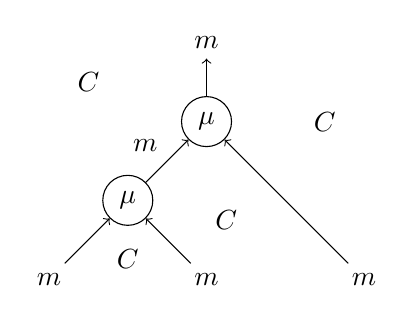
\begin{tikzpicture}[baseline=1.5cm]
\node(f1) at (0,0) {$\mo{m}$};
\node(f2) at (2,0) {$\mo{m}$};
\node(f3) at (4,0) {$\mo{m}$};
\node(n1)[circle,draw] at (1,1) {$\mu$};
\node(n2)[circle,draw] at (2,2) {$\mu$};
\node(f123) at (2,3) {$\mo{m}$};
\draw[->] (f1) -- (n1);
\draw[->] (f2) -- (n1);
\draw[->] (f3) -- (n2);
\draw[->] (n1) -- node(f12)[above left]{$\mo{m}$} (n2);
\draw[->] (n2) -- (f123);
\node at (.5,2.5) {$\ob{C}$};
\node at (1,.25) {$\ob{C}$};
\node at (2.25,.75) {$\ob{C}$};
\node at (3.5,2) {$\ob{C}$};
\end{tikzpicture}
igual a 
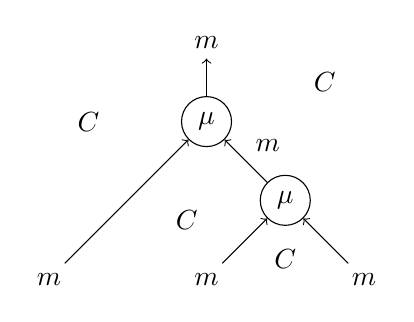
\begin{tikzpicture}[baseline=1.5cm]
\node(f1) at (0,0) {$\mo{m}$};
\node(f2) at (2,0) {$\mo{m}$};
\node(f3) at (4,0) {$\mo{m}$};
\node(n1)[circle,draw] at (3,1) {$\mu$};
\node(n2)[circle,draw] at (2,2) {$\mu$};
\node(f123) at (2,3) {$\mo{m}$};
\draw[->] (f1) -- (n2);
\draw[->] (f2) -- (n1);
\draw[->] (f3) -- (n1);
\draw[->] (n1) -- node(f12)[above right]{$\mo{m}$} (n2);
\draw[->] (n2) -- (f123);
\node at (3.5,2.5) {$\ob{C}$};
\node at (3,.25) {$\ob{C}$};
\node at (1.75,.75) {$\ob{C}$};
\node at (.5,2) {$\ob{C}$};
\end{tikzpicture}
\item Unidad $\eta$ es una 2-cell de $\cat{C}$ desde $\ob{C}$ hasta $\mo{m}$
\item Identidad $\mft{i}$ Es una prueba \\
\begin{tikzpicture}[baseline=(c1.base)]
\node(c1) at (0,0) {$\ob{C}$};
\node(c2) at (4,0) {$\ob{C}$};
\draw[->] (c1) .. controls (1.5,-1.5) and (2.5,-1.5) .. node(f1){} node[below]{$\mo{m}$} (c2);
\draw[->] (c2) .. controls (1.75,-1.5) and (1.75,1.5) .. node(f2){} node[left]{$\mo{m}$} (c2);
\draw[->] (c1) .. controls (1.5,1.5) and (2.5,1.5) .. node(f12){} node[above]{$\mo{m}$} (c2);
\draw[double,double equal sign distance,-implies] (c2) -- node[above]{$\eta$} (f2);
\draw[double,double equal sign distance,-implies] ($(f1.west) !.5! (c2.south)$) .. controls +(-1.5,-.5) and ($(f12.south west) + (-.5,-1)$) .. node[left]{$\mu$} (f12.south west);
\end{tikzpicture}
y
\begin{tikzpicture}[baseline=(c1.base)]
\node(c1) at (0,0) {$\ob{C}$};
\node(c2) at (4,0) {$\ob{C}$};
\draw[->] (c1) .. controls (2.25,1.5) and (2.25,-1.5) .. node(f1){} node[right]{$\mo{m}$} (c1);
\draw[->] (c1) .. controls (1.5,-1.5) and (2.5,-1.5) .. node(f2){} node[below]{$\mo{m}$} (c2);
\draw[->] (c1) .. controls (1.5,1.5) and (2.5,1.5) .. node(f12){} node[above]{$\mo{m}$} (c2);
\draw[double,double equal sign distance,-implies] (c1) -- node[above]{$\eta$} (f1);
\draw[double,double equal sign distance,-implies] ($(f2.east) !.5! (c1.south)$) .. controls +(1.5,-.5) and ($(f12.south east) + (.5,-1)$) .. node[right]{$\mu$} (f12.south east);
\end{tikzpicture}
igual a 
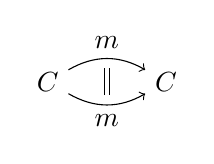
\begin{tikzpicture}[baseline=(c1.base)]
\node(c1) at (0,0) {$\ob{C}$};
\node(c2) at (1.5,0) {$\ob{C}$};
\draw[->] (c1) to[bend right=30] node[below]{$\mo{m}$} node(f1){} (c2);
\draw[->] (c1) to[bend left=30] node[above]{$\mo{m}$} node(f2){} (c2);
\draw[double,double equal sign distance] (f1) -- (f2);
\end{tikzpicture}
\\
Es decir
\begin{tikzpicture}[baseline=1.5cm]
\node(f1) at (0,0) {$\mo{m}$};
\node(n1)[circle,draw] at (1,1) {$\eta$};
\node(n2)[circle,draw] at (0,2) {$\mu$};
\node(f12) at (0,3) {$\mo{m}$};
\draw[->] (f1) -- ++(0,.5) .. controls +(0,.5) and ($(n2.south west) + (-.5,-.5)$) .. (n2.south west);
\draw[->] (n1) -- node[above right]{$\mo{m}$} (n2);
\draw[->] (n2) -- (f12);
\node at (-1,1) {$\ob{C}$};
\node at (1.5,2.25) {$\ob{C}$};
\end{tikzpicture}
y
\begin{tikzpicture}[baseline=1.5cm]
\node(f1) at (0,0) {$\mo{m}$};
\node(n1)[circle,draw] at (-1,1) {$\eta$};
\node(n2)[circle,draw] at (0,2) {$\mu$};
\node(f12) at (0,3) {$\mo{m}$};
\draw[->] (f1) -- ++(0,.5) .. controls +(0,.5) and ($(n2.south east) + (.5,-.5)$) .. (n2.south east);
\draw[->] (n1) -- node[above left]{$\mo{m}$} (n2);
\draw[->] (n2) -- (f12);
\node at (1,1) {$\ob{C}$};
\node at (-1.5,2.25) {$\ob{C}$};
\end{tikzpicture}
igual a
\begin{tikzpicture}[baseline=1.5cm]
\node(f1) at (0,0) {$\mo{m}$};
\node(f2) at (0,3) {$\mo{m}$};
\draw[->] (f1) -- (f2);
\node at (-.5,1.5) {$\ob{C}$};
\node at (.5,1.5) {$\ob{C}$};
\end{tikzpicture}
\end{enumerate}